\documentclass[12pt,letter]{article}
\usepackage{tikz}
\usetikzlibrary{shapes,arrows}
\usepackage{float}
%defining tikz block characteristics
\tikzstyle{block} = [draw, fill=blue!20, rectangle, 
minimum height=3em, minimum width=6em]
\tikzstyle{sum} = [draw, fill=blue!20, circle, node distance=1cm]
\tikzstyle{input} = [coordinate]
\tikzstyle{output} = [coordinate]
\tikzstyle{pinstyle} = [pin edge={to-,thin,black}]

%opening
\title{\textbf{ECE 438 Homework \#4}}
\author{Adam Sumner}
\date{Monday April 13th, 2015}

\begin{document}

\maketitle
\section*{System Diagram}
\begin{figure}[H]
\centering
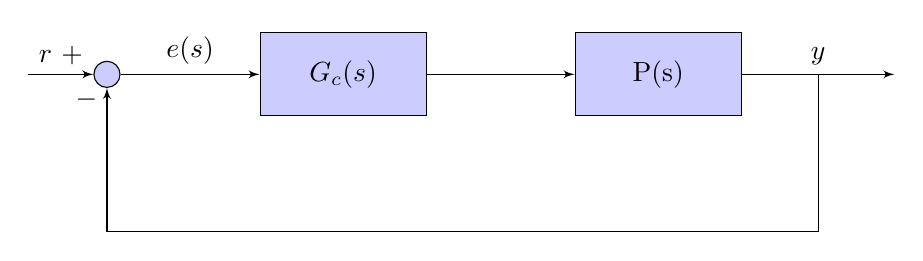
\begin{tikzpicture}[auto, node distance=2cm,>=latex']

% We start by placing the blocks
\node [input, name=input] {};
\node [sum, right of=input] (sum) {};
\node [block, right of =sum, node distance = 3cm] (controller) {$G_c(s)$};
\node [block, right of=controller, node distance=4cm] (system) {P(s)};
% We draw an edge between the controller and system block to 
% calculate the coordinate u. We need it to place the measurement block. 
\draw [->] (controller) -- node[name=u] {} (system);
\node [output, right of=system, node distance = 3cm] (output) {};


% Once the nodes are placed, connecting them is easy. 
\draw [draw,->] (input) -- node {$r$ $+$} (sum);
\draw [->] (sum) -- node {$e(s)$} (controller);
\draw [->] (system) -- node [name=y] {$y$}(output);
\draw [->] (y.south) |- ++(0,-2cm)  -| node[pos=.96]{$-$}(sum) ;
%node [near end] {$y_m$} (sum);
\end{tikzpicture}
\end{figure}
Where: 
		$$P(s)=\frac{K}{s(s+1)(s+10)}$$
\section*{Task 1}

Set $G_{c}(s)=1$ \\
\noindent Transfer Function: 
$$H(s) = \frac{\frac{K}{s(s+1)(s+10)}}{1+\frac{K}{s(s+1)(s+10)}}$$
$$H(s) = \frac{K}{s(s+1)(s+10)+K}$$
Root Locus Form: $$K+s(s+1)(s+10)=0$$
				$$\frac{K}{s(s+1)(s+10)}+1 =0$$
Calculating angles:
$$\phi = \frac{2q+1}{n-m} \cdot 180^{\circ}$$		
$$\phi_{A} = \frac{2(0)+1}{3} \cdot 180 = 60^{\circ}$$	
$$\phi_{B} = \frac{2(1)+1}{3} \cdot 180 = 180^{\circ}$$
$$\phi_{C} = \frac{2(2)+1}{3} \cdot 180 = 300^{\circ}=-60^{\circ}$$	
Centroid:
$$\frac{-10+-1+0}{c}=\frac{-11}{3}\approx -3.667$$		
\begin{figure}[H]
\centering
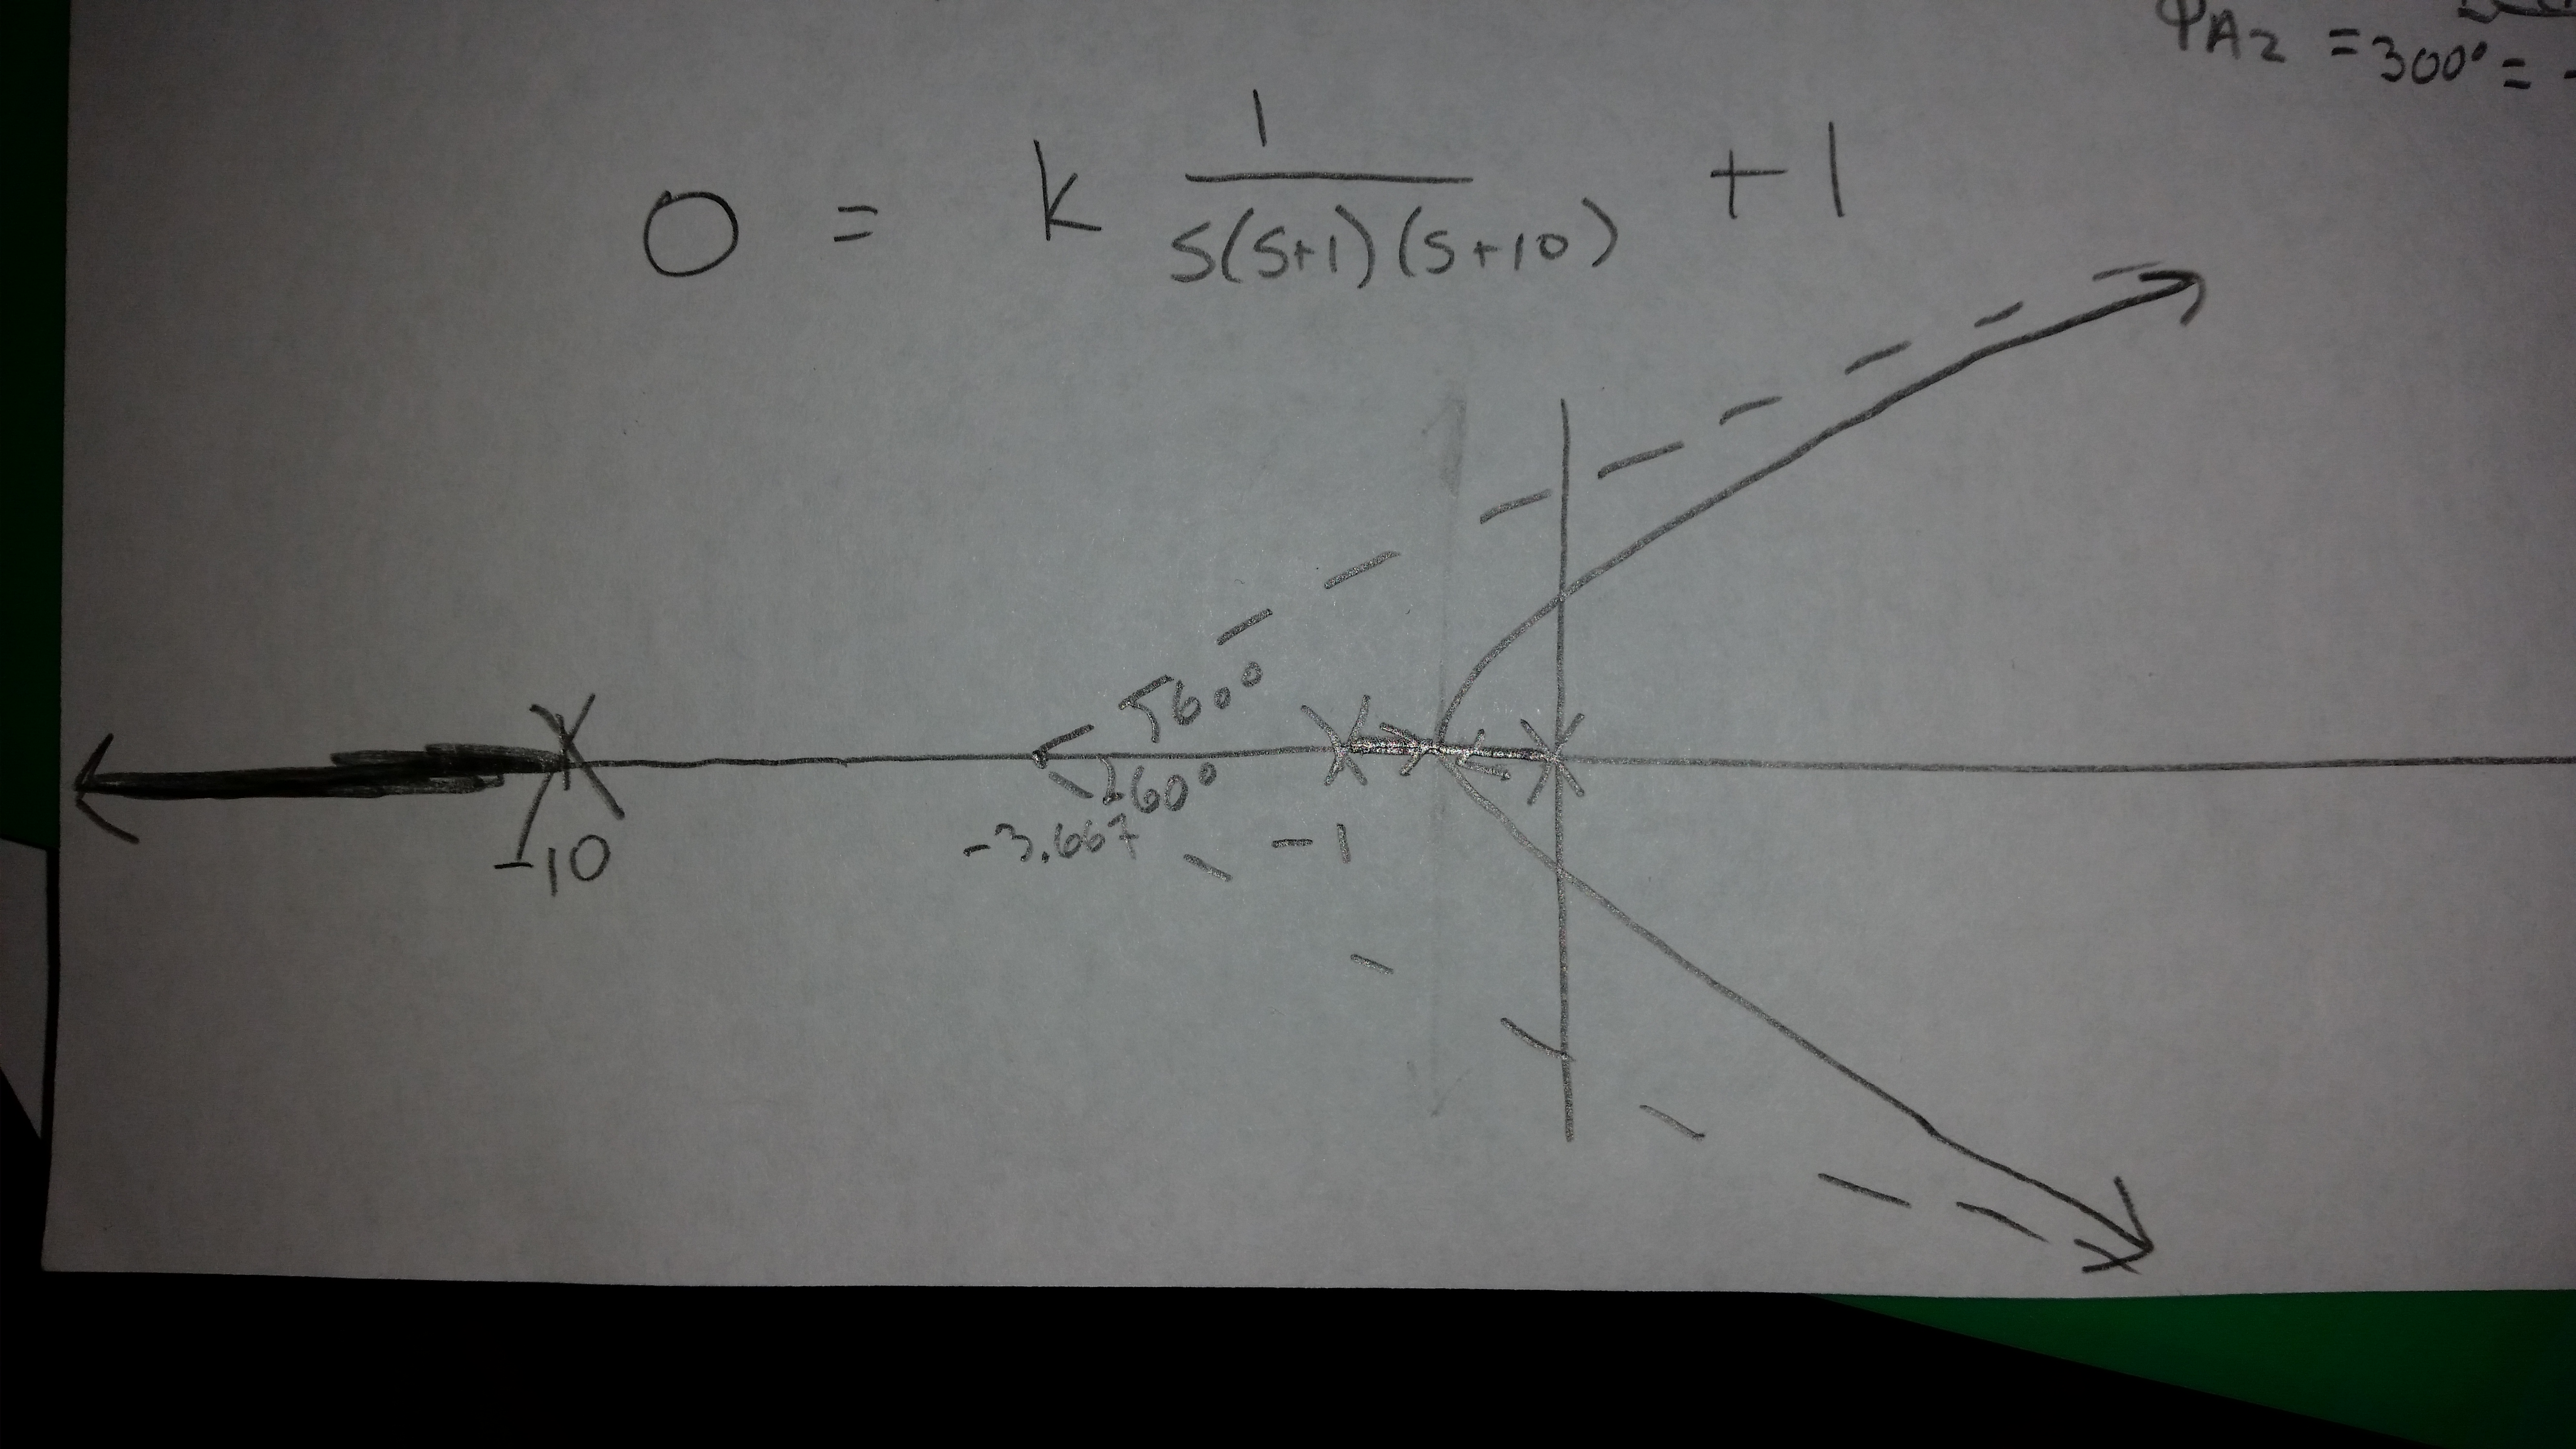
\includegraphics[width=1\linewidth]{20150412_213226}
\caption{Root Locus Sketch}
\label{fig:sketch}
\end{figure}


\begin{figure}[H]
\centering
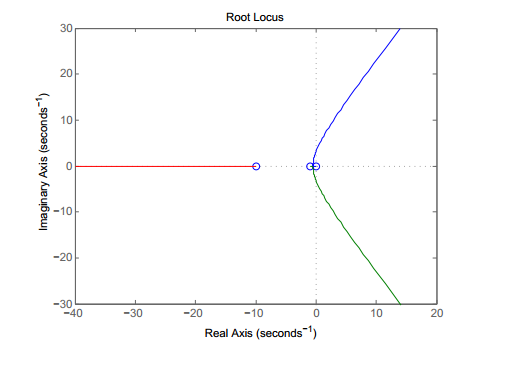
\includegraphics[width=1\linewidth]{rootlocus}
\caption{Matlab Root Locus Sketch}
\label{fig:rootlocus}
\end{figure}
	
\begin{figure}[H]
\centering
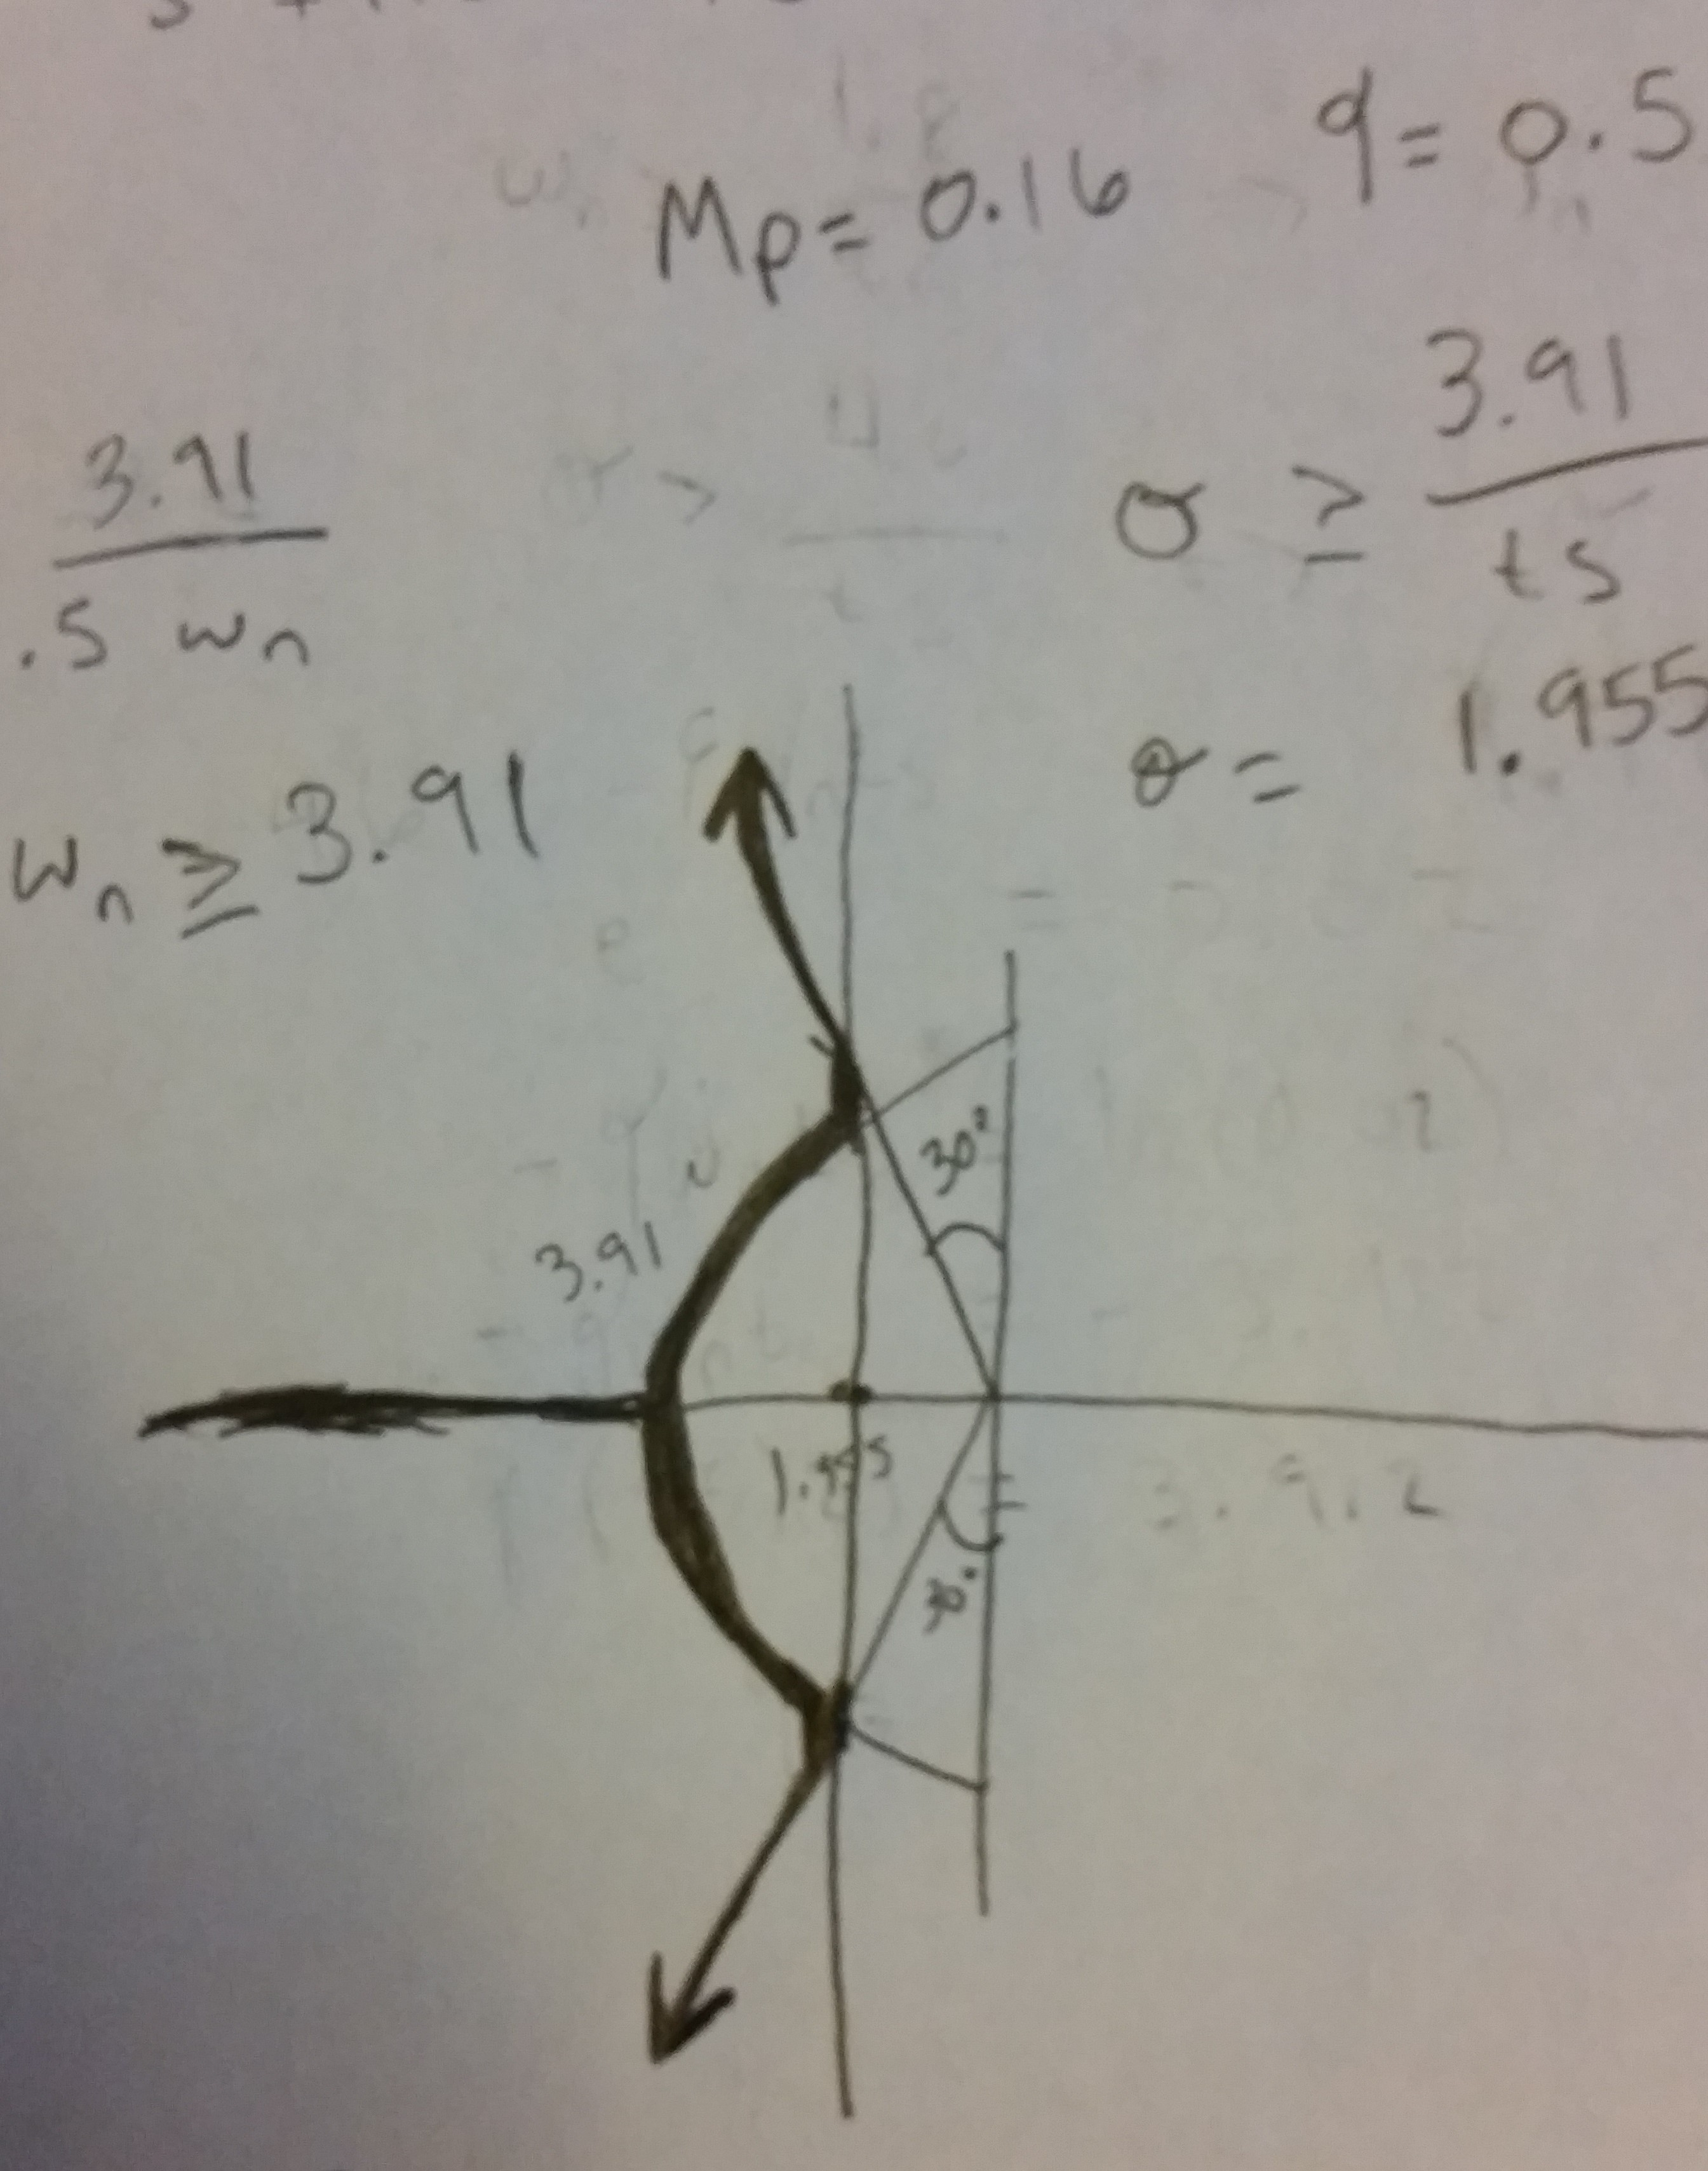
\includegraphics[width=.7\linewidth]{region}
\caption{Region of Operation Sketch}
\label{fig:region}
\end{figure}

\noindent This system without a controller is not possible! No matter what value of $K$ is picked, the transient specifications cannot be met. \\
For $T_r\le0.4s$ $K\approx100$ \\
For $MP\le16\%$ $K\approx8$\\
This is a huge difference.
\section*{Task 2}
The procedure of our controller design will be:
\begin{enumerate}
	\item Analyze current system and understand the desired system requirements
	\item Choose type of controller
	\item Fine tune controller parameters to satisfy system requirements
	\item Produce the desired system performance
\end{enumerate}
Figure \ref{fig:nocontrol} shows the system's step response without a controller implemented.
\begin{figure}[H]
\centering
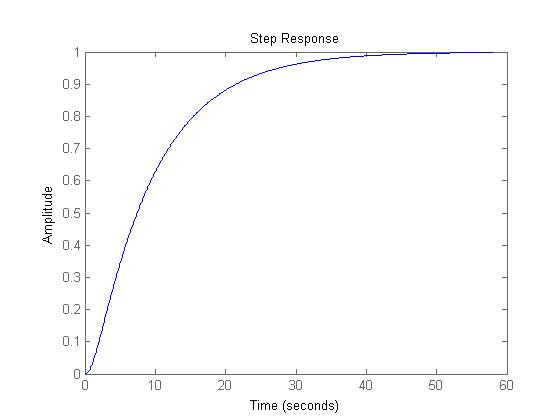
\includegraphics[width=1\linewidth]{nocontrol}
\caption{Step Response Without Controller}
\label{fig:nocontrol}
\end{figure}
\noindent The general type of controller that will be used for the design to meet both dynamic and steady-state performance will be a Proportional Derivative Controller. It has the general form of:
$$D_{c}(s)=k_{p}+k_{D}s$$
This changes the root locus characteristic equation to be of the form:
$$1+K\frac{s+1}{P(s)}=0$$
Where $K=k_{D}$ and arbitrarily selecting the gain ratio as $\frac{k_{p}}{k_{D}}$. Table \ref{tab:param} shows the effect of the controller parameters on the system.
\begin{table}[H]
	\begin{tabular}{|c|c|c|c|c|}
		\hline
		\textbf{Parameter} & \textbf{Rise Time} & \textbf{Overshoot} & \textbf{Settling Time} & \textbf{Steady-State Error} \\ \hline
		$K_p$ & Decrease & Increase & Small Change & Decrease \\ \hline
		$K_i$ & Decrease & Increase & Increase & Eliminate \\ \hline
		$K_d$ & Minor Change & Decrease & Decrease & No Effect \\ \hline
		
	\end{tabular}
	\caption{Effect of Controller Parameter on the System}
	\label{tab:param}
\end{table}
\noindent Upon inspection of Table \ref{tab:param}, it is clear that the parameters of proportional control and derivative control both benefit the system both in transient response and steady state. Looking at Figure \ref{fig:nocontrol}, we can see that the overshoot requirement is met, however, both rise time and settling time are way too high. Proportional control will reduce rise time while increasing overshoot, while Derivative control will reduce the settling time and will counteract the newly gained rise in overshoot.
\\ 
\section*{Task 3}
\noindent To manually tune this system, we first set $K_d$ to 0. We then increase $K_p$ until the output starts to oscillate. From here $K_p$ is set to half that value. Then $K_d$ is increased until the specifications of the system are met.
\\
\noindent $K_p$ was found to be 30 producing these results:
\begin{figure}[H]
\centering
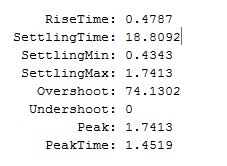
\includegraphics[width=.5\linewidth]{kpresults}
\caption{$K_p$ adjusted results}
\label{fig:kpresults}
\end{figure}

From here, $K_d$ was adjusted to 45 producing these results:
\begin{figure}[H]
\centering
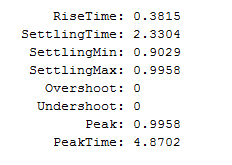
\includegraphics[width=.5\linewidth]{kdresults}
\caption{$K_d$ adjusted results}
\label{fig:kdresults}
\end{figure}

\noindent From here it was then calculated that using a K of 2 produced the correct system requirements. The transient results are shown in Figures \ref{fig:controlledinfo} and \ref{fig:controlledsystem}. The Steady State Error is shown as a constant value with ramp input in Figure \ref{fig:rampstst}. Because it is a Type 1 System, steady state error with step input is 0.
\begin{figure}[H]
\centering
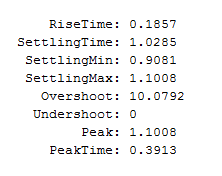
\includegraphics[width=.5\linewidth]{controlledinfo}
\caption{Transient Response Information with Controller}
\label{fig:controlledinfo}
\end{figure}

\begin{figure}[H]
\centering
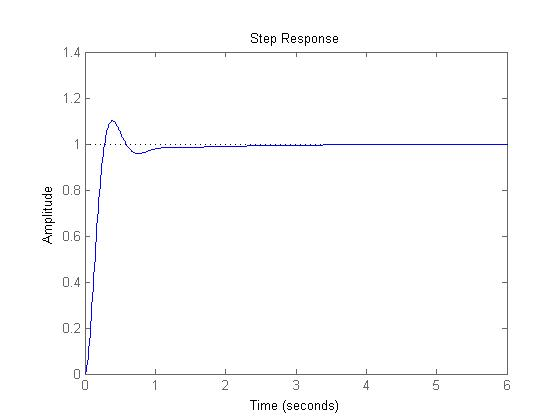
\includegraphics[width=1\linewidth]{controlledsystem}
\caption{Step Response of System with Controller}
\label{fig:controlledsystem}
\end{figure}


\begin{figure}[H]
\centering
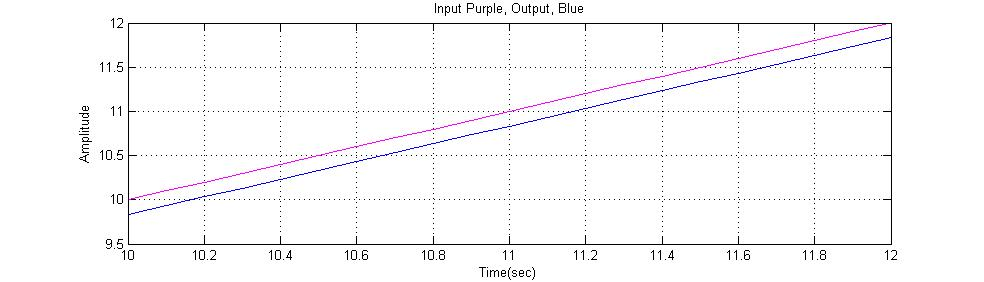
\includegraphics[width=1\linewidth]{rampsteadystateerror}
\caption{Steady State Error with Ramp Input}
\label{fig:rampstst}
\end{figure}

\section*{Task 4}
Figure \ref{fig:controlledrootlocus} shows the Root Locus of the System with the designed controller.
\begin{figure}[H]
\centering
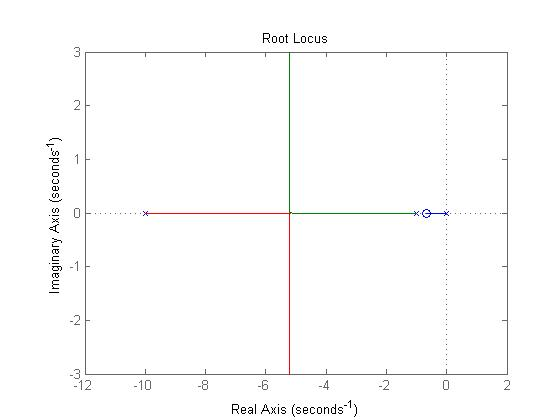
\includegraphics[width=1\linewidth]{controlledrootlocus}
\caption{Root Locus with Control Implementation}
\label{fig:controlledrootlocus}
\end{figure}

\section*{Task 5}
\begin{figure}[H]
\centering
\includegraphics[width=1\linewidth]{"simulink step input"}
\caption{Simulink Step Input}
\label{fig:simulinkstepinput}
\end{figure}
\begin{figure}[H]
\centering
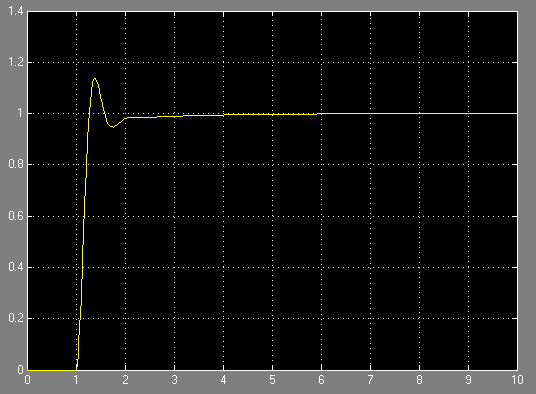
\includegraphics[width=.8\linewidth]{simulinkscope}
\caption{Simulink Output y(t) Scope Results}
\label{fig:simulinkscope}
\end{figure}

As shown previously, Figures \ref{fig:controlledinfo}, \ref{fig:controlledsystem}, and \ref{fig:rampstst} show the simulated values for $y(t)$.
The rise time is 0.1857s, settling time is 1.0285s, overshoot is 10.0792\%, and steady state error is 0 with a step input. These values satisfy our step input specifications.
\section*{Task 6}
\begin{figure}[H]
\centering
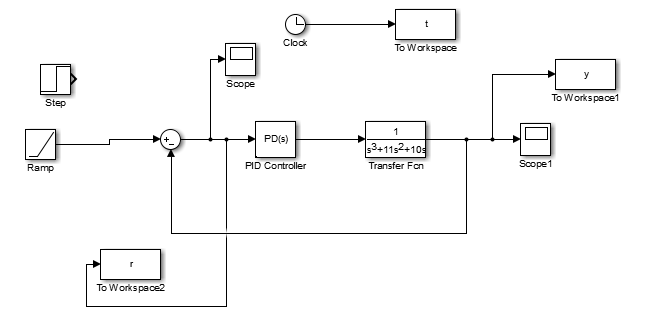
\includegraphics[width=1\linewidth]{rampinput}
\caption{Simulink Model with Ramp Input}
\label{fig:rampinput}
\end{figure}

\begin{figure}[H]
\centering
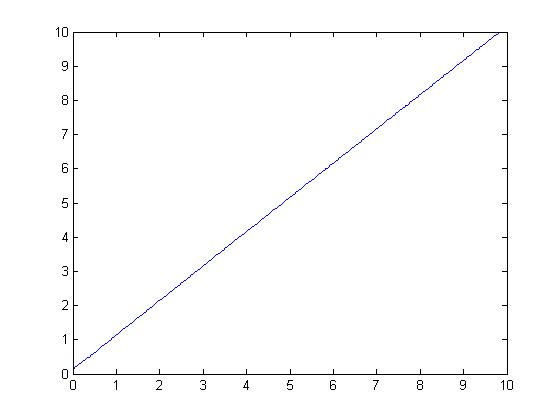
\includegraphics[width=1\linewidth]{rampoutput}
\caption{Ramp Output y(t)}
\label{fig:rampoutput}

\end{figure}
The steady state error was shown previously in Figure \ref{fig:rampstst}. It can be calculated by : 
$$K_v = \lim_{s \to 0} \frac{(30+45s)2s}{s(s+1)(s+10)}$$
$$K_v = 60$$
$$e_{ss} = \frac{1}{K_v} \approx 0.1667$$
Which means that our $e_{ss}$ will be $\le 0.5$, thus satisfying our design constraint.

\section*{Task 7}
I've learned a great deal through the design process of a controller in a unity feedback system. Depending on the specifications of the system, it's important to choose the correct type of controller that will allow you to obtain these results. I plan to improve my learning in this class by doing example problems from the book and reading more examples in real life of actual controller design. 
\end{document}
